%% 
%% Copyright 2007-2020 Elsevier Ltd
%% 
%% This file is part of the 'Elsarticle Bundle'.
%% ---------------------------------------------
%% 
%% It may be distributed under the conditions of the LaTeX Project Public
%% License, either version 1.2 of this license or (at your option) any
%% later version.  The latest version of this license is in
%%    http://www.latex-project.org/lppl.txt
%% and version 1.2 or later is part of all distributions of LaTeX
%% version 1999/12/01 or later.
%% 
%% The list of all files belonging to the 'Elsarticle Bundle' is
%% given in the file `manifest.txt'.
%% 
%% Template article for Elsevier's document class `elsarticle'
%% with harvard style bibliographic references

% \documentclass[preprint,12pt,authoryear]{elsarticle}

%% Use the option review to obtain double line spacing
%% \documentclass[authoryear,preprint,review,12pt]{elsarticle}

%% Use the options 1p,twocolumn; 3p; 3p,twocolumn; 5p; or 5p,twocolumn
%% for a journal layout:
%% \documentclass[final,1p,times,authoryear]{elsarticle}
%% \documentclass[final,1p,times,twocolumn,authoryear]{elsarticle}
\documentclass[final,3p,times,authoryear]{elsarticle}
%% \documentclass[final,3p,times,twocolumn,authoryear]{elsarticle}
% \documentclass[final,5p,times,authoryear]{elsarticle}
 % \documentclass[final,5p,times,twocolumn,authoryear]{elsarticle}

%% For including figures, graphicx.sty has been loaded in
%% elsarticle.cls. If you prefer to use the old commands
%% please give \usepackage{epsfig}

%% The amssymb package provides various useful mathematical symbols
\usepackage{booktabs}
\usepackage{amssymb}
\usepackage{amsmath}
\usepackage{lipsum}
\usepackage{hyperref}
\hypersetup{
    colorlinks=true,
    linkcolor=blue,
    urlcolor=blue,
    citecolor=violet
}
\usepackage{tikz}
\usetikzlibrary{positioning}
\usepackage{subcaption}
% \bibliographystyle{plain}
% \bibliography{references}
%% The amsthm package provides extended theorem environments
%% \usepackage{amsthm}

%% The lineno packages adds line numbers. Start line numbering with
%% \begin{linenumbers}, end it with \end{linenumbers}. Or switch it on
%% for the whole article with \linenumbers.
%% \usepackage{lineno}

%% You might want to define your own abbreviated commands for common used terms, e.g.:
\newcommand{\kms}{km\,s$^{-1}$}
\newcommand{\msun}{$M_\odot}

\journal{Credit Risk Research}


\begin{document}

\begin{frontmatter}

%% Title, authors and addresses

%% use the tnoteref command within \title for footnotes;
%% use the tnotetext command for theassociated footnote;
%% use the fnref command within \author or \affiliation for footnotes;
%% use the fntext command for theassociated footnote;
%% use the corref command within \author for corresponding author footnotes;
%% use the cortext command for theassociated footnote;
%% use the ead command for the email address,
%% and the form \ead[url] for the home page:
%% \title{Title\tnoteref{label1}}
%% \tnotetext[label1]{}
%% \author{Name\corref{cor1}\fnref{label2}}
%% \ead{email address}
%% \ead[url]{home page}
%% \fntext[label2]{}
%% \cortext[cor1]{}
%% \affiliation{organization={},
%%            addressline={}, 
%%            city={},
%%            postcode={}, 
%%            state={},
%%            country={}}
%% \fntext[label3]{}

\title{Transparent Credit Scoring Through Explainable AI }
%% use optional labels to link authors explicitly to addresses:
%% \author[label1,label2]{}
%% \affiliation[label1]{organization={},
%%             addressline={},
%%             city={},
%%             postcode={},
%%             state={},
%%             country={}}
%%
%% \affiliation[label2]{organization={},
%%             addressline={},
%%             city={},
%%             postcode={},
%%             state={},
%%             country={}}

% \author{Anshuman Raj}

\author[1]{Utkarsh Dubey}
\author[1]{Dushyant Bhardwaj}
% \author{Kanishk Sharma}
\author[1]{Kanav Singla}


\affiliation[1]{organization={Department of Computer Science and Engineering, Netaji Subhas University of Technology },%Department and Organization
            addressline={Dwarka}, 
            city={New Delhi},
            country={India}
            }
\begin{abstract}
%% Text of abstract
Despite significant progress in credit-risk prediction, many machine learning models still lack interpretability, limiting their use in high-stakes financial decisions. To address this, we propose \textbf{X-FuzzyScore}, a transparent ensemble framework that integrates fuzzy logic, machine learning, and explainability techniques for credit-risk assessment. The system combines interpretable fuzzy rule-based reasoning with high-accuracy ensemble models \textbf{XGBoost} and \textbf{LightGBM} and employs \textbf{SHAP} and \textbf{LIME} for feature attribution. Trained and evaluated on benchmark datasets including the \textbf{UCI German Credit}, \textbf{UCI Taiwan Credit Card Default}, and \textbf{LendingClub Loan} datasets, the framework follows rigorous preprocessing, normalization, and feature alignment. Experimental results show that X-FuzzyScore achieves superior predictive performance (accuracy, F1-score, AUC) while maintaining interpretability through rule activations and SHAP-based explanations. An interactive visualization dashboard allows stakeholders to explore risk probabilities, linguistic rules, and feature contributions in real time. Overall, X-FuzzyScore offers a robust, explainable solution for credit-risk prediction, enhancing trust and regulatory compliance, with future work focusing on fairness-aware and large-scale real-time extensions.

\end{abstract}

%%Graphical abstract
%\begin{graphicalabstract}
%\includegraphics{grabs}
%\end{graphicalabstract}

%%Research highlights
%\begin{highlights}
%\item Research highlight 1
%\item Research highlight 2
%\end{highlights}

\begin{keyword}
%% keywords here, in the form: keyword \sep keyword, up to a maximum of 6 keywords
explainable AI \sep credit-risk \sep fuzzy logic \sep machine learning \sep SHAP \sep interpretability \sep XGBoost
\sep LightGBM \sep credit scoring \sep transparency

%% PACS codes here, in the form: \PACS code \sep code

%% MSC codes here, in the form: \MSC code \sep code
%% or \MSC[2008] code \sep code (2000 is the default)

\end{keyword}


\end{frontmatter}

%\tableofcontents

%% \linenumbers

%% main text
% Credit Risk Analysis and Prediction Framework
% Introductory Section
% UtkarshDubeyGIT et al.

\section{Introduction}

Credit risk analysis is a cornerstone of modern financial decision-making, directly impacting the stability and profitability of lending institutions. The ability to accurately predict the likelihood of loan default is essential for banks, credit card companies, and fintech organizations. In recent years, the integration of machine learning (ML) and fuzzy logic has enabled the development of more robust, interpretable, and human-centric credit risk models.

This research presents an explainable fuzzy credit-risk prediction framework (X-FuzzyScore) that combines fuzzy reasoning, ML ensemble methods, and explainability techniques (e.g., SHAP) to deliver transparent, actionable insights for credit scoring. The system is designed to:
\begin{itemize}
    \item Predict credit-risk and loan-default probability for individuals and companies.
    \item Provide interpretable predictions in human language and visual formats.
    \item Integrate fuzzy reasoning (e.g., ``high income'', ``medium debt'') with ML accuracy.
    \item Offer a dashboard for model results, fuzzy rules, and SHAP explanations.
\end{itemize}

\subsection{Context and Motivation}

The project aims to address the lack of transparency in traditional credit scoring models by introducing explainable AI (XAI) techniques. 
% The framework leverages multiple datasets (German Credit, Taiwan Credit Card Default, LendingClub Loan Data) to ensure both interpretability and scalability. 
Data preprocessing includes feature alignment, normalization, categorical encoding, and dataset integration.

\subsection{System Architecture}

% \begin{figure}[h]
%     \centering
%     \includegraphics[width=0.9\textwidth]{system_architecture.png}
%     \caption{High-level architecture of the X-FuzzyScore credit risk prediction system.}
% \end{figure}

The architecture consists of:
\begin{enumerate}
    \item Data Preprocessing: Feature alignment, normalization, encoding, and integration.
    \item Fuzzy Layer: Linguistic variable definition and fuzzy rule application.
    \item ML Ensemble Layer: XGBoost, LightGBM, and Random Forest for prediction.
    \item Explainability Layer: SHAP/LIME for feature attribution.
    \item Visualization Frontend: Dashboard with risk gauge, SHAP bar plots, and fuzzy rule viewer.
\end{enumerate}

% \subsection{Dataset Overview}

% \begin{table}[h]
%     \centering
%     \begin{tabular}{|l|l|l|l|}
%         \hline
%         \textbf{Dataset} & \textbf{Source} & \textbf{Size} & \textbf{Use} \\
%         \hline
%         German Credit & UCI ML Repository & $\sim$1,000 & Small interpretable dataset \\
%         Taiwan Credit Card Default & UCI ML Repository & 30,000 & Large-scale testing \\
%         LendingClub Loan Data & Kaggle & 100,000+ & Real-world validation \\
%         \hline
%     \end{tabular}
%     \caption{Datasets used for credit risk analysis.}
% \end{table}

\subsection{Feature Description}

The Taiwan Credit Card Default dataset includes features such as credit limit, sex, education, marriage, age, payment history, bill amounts, and payment amounts. Categorical variables are encoded and outliers are handled during preprocessing. For hybrid models, a fuzzy risk score is added as an additional feature.

\subsection{Mathematical Formulation}

Let $X$ be the feature matrix, $y$ the target (default status), and $f_{ML}$ the machine learning model. The fuzzy risk score $f_{fuzzy}(X)$ is computed using fuzzy rules:
\begin{equation}
    \text{Risk} = f_{ML}(X) + \lambda \cdot f_{fuzzy}(X)
\end{equation}
where $\lambda$ controls the influence of fuzzy logic.

\subsection{Performance Comparison}

\begin{table}[h]
    \centering
    \begin{tabular}{|l|l|l|l|l|l|}
        \hline
        \textbf{Model} & \textbf{Type} & \textbf{Accuracy} & \textbf{Precision} & \textbf{Recall} & \textbf{ROC-AUC} \\
        \hline
        LightGBM + Fuzzy & Hybrid & 0.76 & 0.46 & 0.61 & 0.77 \\
        XGBoost + Fuzzy & Hybrid & 0.76 & 0.46 & 0.61 & 0.77 \\
        RF + Fuzzy & Hybrid & 0.78 & 0.51 & 0.56 & 0.77 \\
        Random Forest & Baseline & 0.78 & 0.50 & 0.55 & 0.77 \\
        Logistic Regression & Baseline & 0.77 & 0.49 & 0.55 & 0.75 \\
        \hline
    \end{tabular}
    \caption{Model performance comparison on Taiwan Credit Card Default dataset.}
\end{table}

% \subsection{Visualization Examples}

% \begin{figure}[h]
%     \centering
%     \includegraphics[width=0.45\textwidth]{default_distribution.png}
%     \includegraphics[width=0.45\textwidth]{education_distribution.png}
%     \caption{Distribution of default payments and education levels.}
% \end{figure}

% \begin{figure}[h]
%     \centering
%     \includegraphics[width=0.45\textwidth]{credit_limit_histogram.png}
%     \includegraphics[width=0.45\textwidth]{credit_limit_boxplot.png}
%     \caption{Credit limit distribution and box plot.}
% \end{figure}

% \begin{figure}[h]
%     \centering
%     \includegraphics[width=0.6\textwidth]{correlation_heatmap.png}
%     \caption{Correlation heatmap of dataset features.}
% \end{figure}

\subsection{Expected Outputs}

\begin{itemize}
    \item Probability: $0.87 \rightarrow 87\%$ chance of repayment
    \item Risk Label: ``Low Risk'', ``Medium Risk'', ``High Risk''
    \item Fuzzy Rules Triggered: ``IF income = high AND debt = low $\rightarrow$ risk = low (activation 0.82)''
    \item SHAP Explanation: income $-0.18$ $\rightarrow$ reduced risk; debt $+0.07$ $\rightarrow$ increased risk
    \item Visualization: Dashboard with gauge, SHAP bars, fuzzy memberships
\end{itemize}


\section{Literature Overview}
\label{literature_overview}

Credit risk assessment is foundational to financial decision-making, and over the decades, a variety of analytical and computational approaches have been developed to predict loan default probability. Traditional models such as Logistic Regression (LR), Linear Discriminant Analysis (LDA), and Decision Trees were widely adopted owing to their interpretability and relatively simple implementation. However, their underlying assumptions—especially linearity and limited capacity to capture complex interactions—restrict their effectiveness on heterogeneous, real-world credit datasets.

With the advent of more powerful Machine Learning techniques, researchers began leveraging models such as Random Forests, Support Vector Machines, Gradient Boosting (particularly XGBoost and LightGBM), and Deep Neural Networks. These approaches have shown substantially better performance on standard credit datasets (e.g., German Credit, Taiwan Credit Card Default, LendingClub), thanks to their ability to automatically learn nonlinear patterns and feature interactions. Nevertheless, such models often operate as ``black boxes,’’ which is problematic in high-stakes domains such as credit, where interpretability, auditability, and regulatory compliance are crucial.

To mitigate the interpretability issue, fuzzy logic–based systems have been applied in credit scoring. Fuzzy Inference Systems (FIS) and Adaptive Neuro-Fuzzy Inference Systems (ANFIS) provide rule-based reasoning using linguistic terms such as ``low-medium income’’ or ``medium-high risk,’’ thereby increasing transparency. Yet, these systems typically require manually defined membership functions and rules, which limits their scalability and adaptability to large, evolving datasets. For example, Piramuthu’s early exploration of neural and neuro-fuzzy methods in credit evaluation \href{https://www.sciencedirect.com/science/article/abs/pii/S0377221797003986}{\textit{Neural networks and neurofuzzy systems for credit risk evaluation}}  demonstrated advantages but also highlighted issues with training complexity and generalization.

Meanwhile, the field of Explainable AI (XAI) has matured significantly, offering tools that aim to render black-box models understandable after the fact. Model-agnostic approaches such as LIME and SHAP assign feature importance values and offer instance-level explanations. In particular, SHAP has gained traction due to its theoretically grounded additive feature attribution framework introduced by Lundberg \& Lee in their paper \href{https://arxiv.org/abs/1705.07874}{\textit{A Unified Approach to Interpreting Model Predictions}}, and its growing use in credit contexts such as \href{https://www.researchgate.net/publication/379068563_Credit_Risk_Prediction_Using_Explainable_AI}{\textit{Credit Risk Prediction Using Explainable AI}}. Recent works like \href{https://www.frontiersin.org/articles/10.3389/frai.2021.752558/full}{}{\textit{SHAP and LIME: An Evaluation in Credit Risk}} 
evaluate the discriminative power and stability of these explainability techniques in financial scenarios.

At the intersection of these paradigms, hybrid and integrated frameworks have been explored to strike a balance between accuracy and interpretability. Neuro-fuzzy or fuzzy-boosting models combine data-driven learning with human-readable rules, and some research layers in SHAP or other XAI methods for post-hoc explanation. For example, \href{https://www.researchgate.net/publication/341032781_A_two-stage_fuzzy_neural_approach_for_credit_risk_assessment_in_a_Brazilian_credit_card_company}{\textit{A Two-Stage Fuzzy Neural Approach for Credit Risk Assessment in a Brazilian Credit Card Company}} illustrates how fuzzy and neural techniques can cooperate. Also, in banking risk modeling, ANFIS has been used to rate risk components in relation to financial performance, as seen in \href{https://www.mdpi.com/2227-9091/13/5/85}{\textit{Rating the Impact of Risks in Banking on Performance}}. However, many existing hybrids do not fully integrate modern XAI tools nor evaluate performance across a consistent set of benchmarks. Furthermore, studies like \href{https://link.springer.com/article/10.1007/s10614-020-10042-0}{\textit{Explainable Machine Learning in Credit Risk Management}} outline ways to make black-box models auditable yet still highlight that achieving interpretability without sacrificing predictive power remains challenging.

In sum, while traditional statistical models offer interpretability and new machine learning methods offer accuracy, and while fuzzy systems introduce human-readability, none fully reconcile all three goals in one framework. Most hybrid works either neglect the integration of XAI, lack consistent benchmarking, or sacrifice one objective for another. This research therefore proposes the \textbf{X-FuzzyScore} framework, which unifies fuzzy rule-based interpretability, ensemble model accuracy, and SHAP-based explanation in a single cohesive system to deliver transparent, trustworthy, and high-performing credit risk predictions.


% Credit Risk Analysis and Prediction Framework
% Methodology Section
% UtkarshDubeyGIT et al.

\section{Methodology}

This section details the end-to-end methodology of the Explainable Fuzzy Credit-Risk Prediction (X-FuzzyScore) framework, covering data preprocessing, fuzzy inference, machine learning models, hybridization strategies, explainability, and evaluation. We emphasize transparent and reproducible practices to ensure both predictive performance and interpretability.

\subsection{Pipeline Overview}

% filepath: /workspaces/Credit-Risk-Analysis-and-Prediction-Framework/Latex/x_fuzzyscore_pipeline_diagram.tex

\begin{figure}[h]
    \centering
    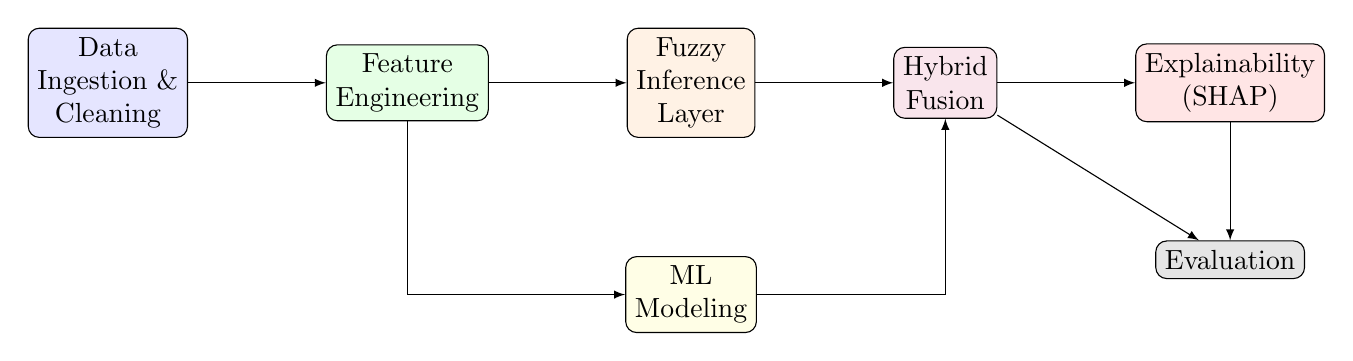
\begin{tikzpicture}[node distance=1.75cm, auto, >=latex, thin]
        % Nodes
        \node[draw, rectangle, rounded corners, fill=blue!10, align=center] (data) {Data \\Ingestion \& \\Cleaning};
        \node[draw, rectangle, rounded corners, fill=green!10, right=of data, align=center] (fe) {Feature \\Engineering};
        \node[draw, rectangle, rounded corners, fill=orange!10, right=of fe, align=center] (fuzzy) {Fuzzy \\Inference \\Layer};
        \node[draw, rectangle, rounded corners, fill=yellow!10, below=1.5cm of fuzzy, align=center] (ml) {ML\\ Modeling};
        \node[draw, rectangle, rounded corners, fill=purple!10, right=of fuzzy, align=center] (hybrid) {Hybrid \\ Fusion};
        \node[draw, rectangle, rounded corners, fill=red!10, right=of hybrid, align=center] (explain) {Explainability \\(SHAP)};
        \node[draw, rectangle, rounded corners, fill=gray!20, below=1.5cm of explain] (eval) {Evaluation};

        % Arrows
        \draw[->] (data) -- (fe);
        \draw[->] (fe) -- (fuzzy);
        \draw[->] (fe) |- (ml);
        \draw[->] (fuzzy) -- (hybrid);
        \draw[->] (ml) -| (hybrid);
        \draw[->] (hybrid) -- (explain);
        \draw[->] (hybrid) -- (eval);
        \draw[->] (explain) -- (eval);
    \end{tikzpicture}
    \caption{X-FuzzyScore Methodology Pipeline: Data preprocessing, feature engineering, fuzzy inference, ML modeling, hybrid fusion, explainability, and evaluation.}
    \label{fig:x_fuzzyscore_pipeline}
\end{figure}

\begin{enumerate}
    \item Data ingestion and cleaning (schema alignment, recoding, deduplication).
    \item Feature engineering (winsorization/capping, scaling if required).
    \item Fuzzy inference layer to compute a human-interpretable risk score.
    \item ML modeling (Logistic Regression, Random Forest, XGBoost, LightGBM).
    \item Hybridization: fuse fuzzy and ML via feature augmentation or late fusion.
    \item Explainability: SHAP-based local and global attributions.
    \item Evaluation: metrics, threshold selection, and calibration checks.
\end{enumerate}

\subsection{Data Preprocessing}

We use the \href{https://archive.ics.uci.edu/dataset/144/statlog+german+credit+data}{UCI Statlog German Credit Data Default} dataset as the primary benchmark.\footnote{\url{https://archive.ics.uci.edu/dataset/144/statlog+german+credit+data}} 
% Let the raw dataset be \(\mathcal{D} = \{(x_i, y_i)\}_{i=1}^N\), where \(y_i \in \{0,1\}\) indicates non-default or default.
\paragraph{Notation.}
We consider a binary classification dataset
\[
\mathcal{D}=\{(x_i,y_i)\}_{i=1}^N,\qquad x_i\in\mathbb{R}^d,\; y_i\in\{0,1\},
\]
where \(y_i=1\) denotes default and \(y_i=0\) non-default. Let
\[
X=\begin{bmatrix}x_1^\top\\ \vdots \\ x_N^\top\end{bmatrix}\in\mathbb{R}^{N\times d},\quad
y=\begin{bmatrix}y_1\\ \vdots \\ y_N\end{bmatrix}\in\{0,1\}^N.
\]

Preprocessing steps (from the EDA notebook):
\begin{itemize}
    \item Column normalization: unify naming (e.g., \texttt{default payment next month} \(\rightarrow\) \texttt{default\_payment}; \texttt{PAY\_0} \(\rightarrow\) \texttt{PAY\_1}) and lowercase all columns.
    \item Categorical recoding: group undocumented categories into ``Others'' (\texttt{education} \(0,5,6\) \(\rightarrow\) 4; \texttt{marriage} \(0\) \(\rightarrow\) 3).
    \item Payment status normalization: map \(-2,-1\) to \(0\) in \texttt{pay\_1}--\texttt{pay\_6} to represent no-consumption or paid-in-full as non-delinquency.
    \item Deduplication: drop duplicates after normalization to avoid leakage and inflated support.
    \item Outlier handling: for heavy-tailed features (\texttt{limit\_bal}, \texttt{bill\_amt\*}, \texttt{pay\_amt\*}), apply upper capping (winsorization) to obtain features like \texttt{limit\_bal\_capped}, \texttt{bill\_amt1\_capped}, ... \footnote{We assume percentile-based capping (e.g., 1st--99th) consistent with the feature names; exact cutoffs are recorded in the preprocessing notebook.}
\end{itemize}

We use an 80/20 train-test split (\(n_{train}=23971\), \(n_{test}=5993\)) consistent with reported metrics. Class imbalance is addressed during evaluation via threshold tuning and by optionally using class-weighted losses in ML models.

\subsection{Fuzzy Inference Layer}

The fuzzy layer provides a human-interpretable risk score \(s_{\text{fuzzy}} \in [0,1]\). We define linguistic variables over selected features (e.g., credit limit, bill amounts, delinquency, payment ratios), each with membership functions for labels such as Low, Medium, and High.

\subsubsection{Membership Functions}

For a scalar feature \(x\), a triangular membership function for label \(\ell\) is:
\begin{equation}
    \mu_{\ell}(x; a,b,c) = \max\left(\min\left(\frac{x-a}{b-a}, \frac{c-x}{c-b}\right), 0\right),\; a < b < c.
\end{equation}
Trapezoidal sets \(\mu_{\ell}(x; a,b,c,d)\) generalize plateaus in the core. Parameters are chosen from quantiles of the training data or domain guidelines.

% \begin{figure}[h]
%     \centering
%     % Example fuzzy membership illustration (placeholder from EDA images)
%     \includegraphics[width=0.75\textwidth]{./figures/process1_img_002.png}
%     \caption{Example membership-like curves used illustratively. Replace with exact fuzzy membership plots if generated.}
% \end{figure}

\subsubsection{Rule Base and Inference}

We use Mamdani inference with min (\(\wedge\)) as the t-norm and max (\(\vee\)) as the s-norm. Example rules:
\begin{align}
    &\textbf{R1:}\; \text{IF } \text{limit\_bal is Low} \wedge \text{delinquency is High} \Rightarrow \text{risk is High},\\
    &\textbf{R2:}\; \text{IF } \text{bill utilization is Low} \wedge \text{payment history is Good} \Rightarrow \text{risk is Low}.
\end{align}
For a rule with antecedent membership \(\alpha\), the implied consequent set is clipped: \(\mu_{C'}(z) = \min(\alpha, \mu_C(z))\). Aggregation across rules uses max. Defuzzification via centroid yields:
\begin{equation}
    s_{\text{fuzzy}} = \frac{\int z\, \mu_{\text{agg}}(z)\,dz}{\int \mu_{\text{agg}}(z)\,dz},\quad z \in [0,1].
\end{equation}

% \begin{figure}[h]
%     \centering
%     % Placeholder for fuzzy rules workflow
%     \includegraphics[width=0.75\textwidth]{./figures/process1_img_003.png}
%     \caption{Illustration of the inference workflow (placeholder). Replace with a dedicated fuzzy rules diagram if available.}
% \end{figure}

\subsection{Machine Learning Models}

We train standard classifiers on engineered features (23 baseline features) and on the hybrid set that appends \(s_{\text{fuzzy}}\) (24 features). Let \(x \in \mathbb{R}^d\), \(y \in \{0,1\}\).

\paragraph{Logistic Regression} predicts \(p(y=1\mid x) = \sigma(w^\top x + b)\), \(\sigma(t) = 1/(1+e^{-t})\), with parameters learned via cross-entropy minimization and L2 regularization.

\paragraph{Random Forest} aggregates \(T\) decision trees \(\{h_t\}\) trained on bootstraps and feature subsamples; prediction is the average of tree posteriors.

\paragraph{Gradient Boosting (XGBoost/LightGBM)} optimizes an additive tree ensemble \(F_M(x) = \sum_{m=1}^M \gamma_m h_m(x)\) via gradient descent on a differentiable objective (logistic loss with regularization), using histogram-based splits and shrinkage.

\subsection{Hybridization Strategies}

We combine fuzzy and ML predictions in two complementary ways:
\begin{description}
    \item[Feature Augmentation:] concatenate the fuzzy score to the feature vector: \(x' = [x; s_{\text{fuzzy}}]\). The classifier learns to weight \(s_{\text{fuzzy}}\) with other features.
    \item[Late Fusion:] combine calibrated posteriors: \(\hat{p} = (1-\lambda)\, p_{\text{ML}} + \lambda\, s_{\text{fuzzy}}\), \(\lambda \in [0,1]\) tuned on validation data, or learn a meta-learner \(g\big(p_{\text{ML}}, s_{\text{fuzzy}}\big)\).
\end{description}

\subsection{Explainability with SHAP}

We adopt SHAP, an additive feature attribution method with explanations of the form \(f(x) \approx \phi_0 + \sum_i \phi_i\). Here, \(\phi_i\) is the Shapley value for feature \(i\), computed from coalitional contributions. We report global importance via mean \(|\phi_i|\) and local explanations for individual decisions (especially near the decision threshold).

% \begin{figure}[h]
%     \centering
%     % Placeholder for SHAP outputs
%     \includegraphics[width=0.75\textwidth]{./figures/process1_img_004.png}
%     \caption{Example explanation-style plot (placeholder). Replace with SHAP summary and force plots when generated.}
% \end{figure}

\subsection{Representative EDA Visuals}

We include representative plots extracted from the EDA notebook to ground the methodology and preprocessing choices:

% \begin{figure}[h]
%     \centering
%     \begin{subfigure}[b]{0.48\textwidth}
%         \centering
%         \includegraphics[width=\textwidth]{./figures/process1_img_005.png}
%         \caption{Default vs non-default distribution}
%     \end{subfigure}
%     \hfill
%     \begin{subfigure}[b]{0.48\textwidth}
%         \centering
%         \includegraphics[width=\textwidth]{./figures/process1_img_006.png}
%         \caption{Education level distribution}
%     \end{subfigure}
%     \caption{Target imbalance and categorical distribution motivate threshold tuning and careful encoding.}
% \end{figure}

% \begin{figure}[h]
%     \centering
%     \begin{subfigure}[b]{0.48\textwidth}
%         \centering
%         \includegraphics[width=\textwidth]{./figures/process1_img_007.png}
%         \caption{Credit limit histogram}
%     \end{subfigure}
%     \hfill
%     \begin{subfigure}[b]{0.48\textwidth}
%         \centering
%         \includegraphics[width=\textwidth]{./figures/process1_img_008.png}
%         \caption{Credit limit boxplot}
%     \end{subfigure}
%     \caption{Right-skew and outliers motivate winsorization/capping strategies.}
% \end{figure}

% \begin{figure}[h]
%     \centering
%     \includegraphics[width=0.8\textwidth]{./figures/process1_img_009.png}
%     \caption{Correlation heatmap indicating strong temporal correlations among bill amount features.}
% \end{figure}

\subsection{Evaluation Protocol}

\paragraph{Split and Metrics} We evaluate on a held-out test set (\(20\%\)). Metrics include Accuracy, Precision, Recall, F1, and ROC-AUC:
\begin{align}
    \text{Precision} &= \frac{TP}{TP + FP},\quad \text{Recall} = \frac{TP}{TP + FN},\\
    \text{F1} &= 2\,\frac{\text{Precision} \cdot \text{Recall}}{\text{Precision} + \text{Recall}},\quad \text{AUC} = \int_0^1 \text{TPR}(\text{FPR})\,d\,\text{FPR}.
\end{align}

\paragraph{Thresholding and Imbalance} Because defaults are the minority class, we tune the decision threshold \(\tau\) to optimize F1 or Youden's \(J = \text{TPR} - \text{FPR}\). We also consider class-weighted losses and probability calibration checks (e.g., reliability curves).

\paragraph{Reported Results} On the Taiwan dataset, the best-performing hybrids achieve ROC-AUC around 0.77 with Recall around 0.60 (e.g., LightGBM+Fuzzy and XGBoost+Fuzzy), while Random Forest baselines attain similar AUC but slightly different precision-recall trade-offs.

\subsection{Reproducibility}

We fix random seeds, log preprocessing parameters (e.g., capping percentiles), and record feature schemas. The hybrid feature set includes the fuzzy score, yielding 24 features total, with baseline features numbering 23. Train/test sizes are fixed at \(23971/5993\) for comparability.

\subsection{Computational Considerations}

Tree ensembles scale approximately with \(\mathcal{O}(M\, d\, n \log n)\) for \(M\) trees and \(n\) samples. Fuzzy inference is linear in the number of rules and variables. The overhead of SHAP (TreeSHAP) is polynomial in tree depth and tree count but efficient for tree models.

\subsection{Method Summary}

The methodology tightly integrates interpretable fuzzy reasoning with strong ML classifiers, combining human-understandable rule-based insights with data-driven accuracy. The hybridization improves recall while maintaining competitive AUC, and SHAP provides transparent explanations for stakeholders and regulators.

\subsection{Training Configuration and Hyperparameters}

Unless otherwise specified, models are trained with the following default settings (tuned via validation or simple grid search):
\begin{itemize}
    \item Logistic Regression: penalty=L2, $C \in \{0.1, 1, 10\}$, class\_weight=\texttt{balanced} (optional).
    \item Random Forest: $n$\_estimators $\in [200, 600]$, max\_depth $\in \{None, 8, 12\}$, max\_features=sqrt.
    \item XGBoost/LightGBM: learning\_rate $\in [0.03, 0.1]$, n\_estimators $\in [300, 800]$, max\_depth $\in \{4,6,8\}$, subsample/colsample\_by\_tree $\in [0.6, 0.9]$.
    \item Fuzzy layer: membership parameters derived from quantiles (e.g., 20/50/80th), rule base curated to cover high-risk and low-risk archetypes.
\end{itemize}

Feature scaling is not mandatory for tree models; for LR, we use either standardization or leave raw if features are capped and numerically stable. Categorical features (e.g., \texttt{sex}, \texttt{education}, \texttt{marriage}) are kept as integers, consistent with domain semantics.

\subsection{Leakage Prevention and Validation}

All preprocessing (including capping percentiles and membership calibration) is performed within the training data scope and applied to the test set using frozen parameters to prevent leakage. Validation strategies considered:
\begin{itemize}
    \item Hold-out: 80/20 split as reported.
    \item 5-fold cross-validation for hyperparameter tuning; final metrics reported on the hold-out test.
    \item Temporal awareness: although the dataset is static, the payment history order is preserved; no target leakage features are introduced.
\end{itemize}

\subsection{Calibration and Threshold Selection}

We optionally apply Platt scaling or isotonic regression to calibrate tree ensemble probabilities. Threshold \(\tau\) is selected to maximize F1 or based on application utility (e.g., cost-sensitive thresholding):
\begin{equation}
    	au^* = \arg\max_{\tau} \; U(\text{TP}(\tau), \text{FP}(\tau), \text{FN}(\tau)),
\end{equation}
where $U$ encodes operational costs/benefits.

\subsection{Uncertainty and Statistical Testing}

We compute 95\% confidence intervals via stratified bootstrap (1{,}000 resamples) for AUC and F1. For model comparisons, we report paired bootstrap $p$-values or DeLong's test for ROC-AUC when applicable.

\subsection{Algorithmic Summaries}

\paragraph{Fuzzy Inference (Mamdani)}
\begin{enumerate}
    \item Compute antecedent memberships for selected features.
    \item Evaluate each rule with t-norm (min) to get activation $\alpha$.
    \item Clip consequent set by $\alpha$ and aggregate via s-norm (max).
    \item Defuzzify aggregated set by centroid to obtain $s_{\text{fuzzy}}$.
\end{enumerate}

\paragraph{Hybrid Late Fusion}
\begin{enumerate}
    \item Train ML model to obtain $p_{\text{ML}}(x)$.
    \item Compute $s_{\text{fuzzy}}(x)$ from fuzzy layer.
    \item Combine $\hat{p}(x) = (1-\lambda)\, p_{\text{ML}}(x) + \lambda\, s_{\text{fuzzy}}(x)$; tune $\lambda$ on validation.
\end{enumerate}

\subsection{Feature Overview}

Table~\ref{tab:feat} summarizes the primary engineered features; the hybrid setting appends the fuzzy risk score.
\begin{table}[h]
    \centering
    \begin{tabular}{ll}
        	
        	\textbf{Feature group} & \textbf{Examples} \\
        \midrule
        Demographics & \texttt{sex}, \texttt{education}, \texttt{marriage}, \texttt{age} \\
        Credit limit & \texttt{limit\_bal\_capped} \\
        Payment status & \texttt{pay\_1} -- \texttt{pay\_6} (normalized) \\
        Bill amounts & \texttt{bill\_amt1\_capped} -- \texttt{bill\_amt6\_capped} \\
        Payment amounts & \texttt{pay\_amt1\_capped} -- \texttt{pay\_amt6\_capped} \\
        Hybrid addition & \texttt{fuzzy\_risk\_score} \\
        \bottomrule
    \end{tabular}
    \caption{Feature overview (baseline: 23 features; hybrid: +1 fuzzy risk score).}
    \label{tab:feat}
\end{table}


% %%\label{}
% \lipsum[2]

% \subsection{Subsection title}
% \lipsum[3]

% \begin{table}
% \begin{tabular}{l c c c} 
%  \hline
%  Source & RA (J2000) & DEC (J2000) & $V_{\rm sys}$ \\ 
%         & [h,m,s]    & [o,','']    & \kms          \\
%  \hline
%  NGC\,253 & 	00:47:33.120 & -25:17:17.59 & $235 \pm 1$ \\ 
%  M\,82 & 09:55:52.725, & +69:40:45.78 & $269 \pm 2$ 	 \\ 
%  \hline
% \end{tabular}
% \caption{Random table with galaxies coordinates and velocities, Number the tables consecutively in
% accordance with their appearance in the text and place any table notes below the table body. Please avoid using vertical rules and shading in table cells.
% }
% \label{Table1}
% \end{table}


% \section{Discussion}
% %%\label{}
% \lipsum[4]

% \section{Summary and conclusions}
% %%\label{}
% \lipsum[1-4]


% \section*{Acknowledgements}
% Thanks to ...

% %% The Appendices part is started with the command \appendix;
% %% appendix sections are then done as normal sections
% \appendix

% \section{Appendix title 1}
% %% \label{}

% \section{Appendix title 2}

\begin{thebibliography}{00}

\bibitem[Zhou and Wang(2025)]{zhou2025enhancing}
Zhou, G. and Wang, S., 2025. Enhancing Credit Risk Decision-Making in Supply Chain Finance With Interpretable Machine Learning Model. \textit{IEEE Access}, 13, 14239–14251. doi:10.1109/ACCESS.2025.3530433.

\bibitem[Mashrur et al.(2020)]{mashrur2020machine}
Mashrur, A., Luo, W., Zaidi, N. A., and Robles-Kelly, A., 2020. Machine Learning for Financial Risk Management: A Survey. \textit{IEEE Access}, 8, 203203–203223. doi:10.1109/ACCESS.2020.3036322.

\bibitem[Song et al.(2024)]{song2024credit}
Song, M., Ma, H., Zhu, Y., and Zhang, M., 2024. Credit Risk Prediction Based on Improved ADASYN Sampling and Optimized LightGBM. \textit{Journal of Social Computing}, 5(3), 232–241. doi:10.23919/JSC.2024.0019.

\bibitem[Kumar et al.(2023)]{kumar2023ai}
Kumar, V., Saheb, S. S., Preeti, Ghayas, A., Kumari, S., Chandel, J. K., Pandey, S. K., and Kumar, S., 2023. AI-Based Hybrid Models for Predicting Loan Risk in the Banking Sector. \textit{Big Data Mining and Analytics}, 6(4), 478–490. doi:10.26599/BDMA.2022.9020037.

\bibitem[Song and Peng(2019)]{song2019mcdm}
Song, Y. and Peng, Y., 2019. A MCDM-Based Evaluation Approach for Imbalanced Classification Methods in Financial Risk Prediction. \textit{IEEE Access}, 7, 84897–84907. doi:10.1109/ACCESS.2019.2924923.

\bibitem[Alam et al.(2020)]{alam2020investigation}
Alam, T. M., Shaukat, K., Hameed, I. A., Luo, S., Sarwar, M. U., Shabbir, S., Li, J., and Khushi, M., 2020. An Investigation of Credit Card Default Prediction in the Imbalanced Datasets. \textit{IEEE Access}, 8, 201173–201198. doi:10.1109/ACCESS.2020.3033784.

\bibitem[Kisten and Khosa(2024)]{kisten2024enhancing}
Kisten, M. and Khosa, M., 2024. Enhancing Fairness in Credit Assessment: Mitigation Strategies and Implementation. \textit{IEEE Access}, 12, 177277–177284. doi:10.1109/ACCESS.2024.3505836.

\end{thebibliography}

%% \label{}

%% If you have bibdatabase file and want bibtex to generate the
%% bibitems, please use
%%

% \bibliographystyle{IEEEtran}
% \bibliography{references}

%% else use the following coding to input the bibitems directly in the
%% TeX file.

%%\begin{thebibliography}{00}

%% \bibitem[Author(year)]{label}
%% For example:

%% \bibitem[Aladro et al.(2015)]{Aladro15} Aladro, R., Martín, S., Riquelme, D., et al. 2015, \aas, 579, A101


%%\end{thebibliography}

\end{document}

\endinput
%%
%% End of file `elsarticle-template-harv.tex'.
